\documentclass[a4paper,showframe,11pt]{report}\usepackage[]{graphicx}\usepackage[]{color}
%% maxwidth is the original width if it is less than linewidth
%% otherwise use linewidth (to make sure the graphics do not exceed the margin)
\makeatletter
\def\maxwidth{ %
  \ifdim\Gin@nat@width>\linewidth
    \linewidth
  \else
    \Gin@nat@width
  \fi
}
\makeatother

\definecolor{fgcolor}{rgb}{0.196, 0.196, 0.196}
\newcommand{\hlnum}[1]{\textcolor[rgb]{0.063,0.58,0.627}{#1}}%
\newcommand{\hlstr}[1]{\textcolor[rgb]{0.063,0.58,0.627}{#1}}%
\newcommand{\hlcom}[1]{\textcolor[rgb]{0.588,0.588,0.588}{#1}}%
\newcommand{\hlopt}[1]{\textcolor[rgb]{0.196,0.196,0.196}{#1}}%
\newcommand{\hlstd}[1]{\textcolor[rgb]{0.196,0.196,0.196}{#1}}%
\newcommand{\hlkwa}[1]{\textcolor[rgb]{0.231,0.416,0.784}{#1}}%
\newcommand{\hlkwb}[1]{\textcolor[rgb]{0.627,0,0.314}{#1}}%
\newcommand{\hlkwc}[1]{\textcolor[rgb]{0,0.631,0.314}{#1}}%
\newcommand{\hlkwd}[1]{\textcolor[rgb]{0.78,0.227,0.412}{#1}}%
\let\hlipl\hlkwb

\usepackage{framed}
\makeatletter
\newenvironment{kframe}{%
 \def\at@end@of@kframe{}%
 \ifinner\ifhmode%
  \def\at@end@of@kframe{\end{minipage}}%
  \begin{minipage}{\columnwidth}%
 \fi\fi%
 \def\FrameCommand##1{\hskip\@totalleftmargin \hskip-\fboxsep
 \colorbox{shadecolor}{##1}\hskip-\fboxsep
     % There is no \\@totalrightmargin, so:
     \hskip-\linewidth \hskip-\@totalleftmargin \hskip\columnwidth}%
 \MakeFramed {\advance\hsize-\width
   \@totalleftmargin\z@ \linewidth\hsize
   \@setminipage}}%
 {\par\unskip\endMakeFramed%
 \at@end@of@kframe}
\makeatother

\definecolor{shadecolor}{rgb}{.97, .97, .97}
\definecolor{messagecolor}{rgb}{0, 0, 0}
\definecolor{warningcolor}{rgb}{1, 0, 1}
\definecolor{errorcolor}{rgb}{1, 0, 0}
\newenvironment{knitrout}{}{} % an empty environment to be redefined in TeX

\usepackage{alltt}
\usepackage{standalone}
\standalonetrue
\ifstandalone
  \usepackage{../../haziq_thesis}
  \usepackage{../../haziq_maths}
  \usepackage{../../haziq_glossary}
  \addbibresource{../../bib/haziq.bib}
  \externaldocument{../01/.texpadtmp/introduction}
\fi




\IfFileExists{upquote.sty}{\usepackage{upquote}}{}
\begin{document}

We consider a balanced longitudinal data set consisting of weights in kilograms of 60 cows, 30 of which were randomly assigned to treatment group A, and the remaining 30 to treatment group B. The animals were weighed 11 times over a 133-day period; the first 10 measurements for each animal were made at two-week intervals and the last measurement was made one week later. This experiment was reported by cite{kenward1987method}, and the data set is included as part of the package \pkg{jmcm} in \proglang{R}.

\begin{knitrout}
\definecolor{shadecolor}{rgb}{1, 1, 1}\color{fgcolor}\begin{kframe}
\begin{alltt}
\hlstd{R> }\hlkwd{data}\hlstd{(cattle,} \hlkwc{package} \hlstd{=} \hlstr{"jmcm"}\hlstd{)}
\end{alltt}
\begin{verbatim}
## # A tibble: 660 x 4
##        id  time  group weight
##    <fctr> <dbl> <fctr>  <int>
##  1      1     0      A    233
##  2      1    14      A    224
##  3      1    28      A    245
##  4      1    42      A    258
##  5      1    56      A    271
##  6      1    70      A    287
##  7      1    84      A    287
##  8      1    98      A    287
##  9      1   112      A    290
## 10      1   126      A    293
## # ... with 650 more rows
\end{verbatim}
\end{kframe}
\end{knitrout}

The response variable of interest are the \code{weight} growth curves, and the aim is to investigate whether a treatment effect is present. The usual approach to analyse a longitudinal data set such as this one is to assume that the observed growth curves are realizations of a Gaussian process. For example, cite{kenward1987method} assumed a so-called ante-dependence structure of order $k$, which assumes an observation depends on the previous $k$ observations, but given these, is independent of any preceeding observations.

Using the I-prior, it is not necessary to assume the growth curves were drawn randomly. Instead, it suffices to assume that they lie in an appropriate function class. For this example, we assume that the function class is the FBM RKHS, i.e., we assume a smooth effect of time on weight. The growth curves form a multidimensional (or functional) response equivalent to a ``wide'' format of representing repeated measures data. In our analysis using the \pkg{iprior} package, we used the ``long'' format and thus our (unidimensional) sample size $n$ is equal to $60$ cows $\times$ $11$ repeated measurements. We also have two covariates potentially influencing growth, namely the cow subject \code{id} and also treatment \code{group}. The regression model can be thought of as
\[
  \text{\code{weight}} = f(\text{\code{id}}, \, \text{\code{group}}, \, \text{\code{time}}) + \text{error}.
\]

We assume iid errors, and in addition to a smooth effect of \code{time}, we further assume a nominal effect of both cow \code{id} and treatment \code{group} using the Pearson RKHS. In the \pkg{iprior} package, factor type objects are treated with the Pearson kernel automatically, and the only \code{model} option we need to specify is the \code{kernel = "FBM"} option for the \code{time} variable. We have opted not to estimate the Hurst coefficient in the interest of computational time, and instead left it at the default value of 0.5. Table \ref{tab:cowmodel} explains the five models we have fitted.

\begin{table}[ht]
\centering
\begin{tabular}{lp{6cm}l}
\toprule
Model & Explanation & Formula (\verb@weight ~ ...@)                              \\
\midrule
1     & Growth does not vary with treatment nor among cows                                                         & \verb@time@                \\
\Top
2     & Growth varies among cows only                                                                              & \verb@id * time@             \\
\Top
3     & Growth varies with treatment only                                                                          & \verb@group * time@           \\
\Top
4     & Growth varies with treatment and among cows                                                                & \verb@id * time + group * time@ \\
\Top
5     & Growth varies with treatment and among cows, with an interaction effect between treatment and cow & \verb@id * group * time@ \\
\bottomrule
\end{tabular}
\caption{A brief description of the five models fitted using I-priors.}
\label{tab:cowmodel}
\end{table}

The simplest model fitted was one in which the growth curves do not depend on the treatment effect or individual cows. We then added treatment effect and the cow \code{id} as covariates, separately first and then together at once. We also assumed that both of these covariates are time-varying, and hence added also the interaction between these covariates and the \code{time} variable. The final model was one in which an interaction between treatment effect and individual cows was assumed, which varied over time.

 All models were first loaded into a \code{ipriorKernel} object, and then fitted using the \code{ipriorOptim} function. Compared to the EM algorithm alone, we found that the combination of direct optimization with the EM algorithm in the \code{ipriorOptim} routine fits the model about six times faster for this data set due to slow convergence of EM algorithm. Here is the code and output for fitting the first model.


\begin{knitrout}
\definecolor{shadecolor}{rgb}{1, 1, 1}\color{fgcolor}\begin{kframe}
\begin{alltt}
\hlstd{R> }\hlstd{mod1} \hlkwb{<-} \hlkwd{kernL}\hlstd{(weight} \hlopt{~} \hlstd{time,} \hlkwc{data} \hlstd{= cattle,} \hlkwc{model} \hlstd{=} \hlkwd{list}\hlstd{(}\hlkwc{kernel} \hlstd{=} \hlstr{"FBM"}\hlstd{))}
\hlstd{R> }\hlstd{mod1.fit} \hlkwb{<-} \hlkwd{ipriorOptim}\hlstd{(mod1)}
\end{alltt}
\begin{verbatim}
## Iteration 0:    Log-likelihood = -40740.339 
## Iteration 1:    Log-likelihood = -5416.4625 .......
## Iteration 2:    Log-likelihood = -3347.1579 .......
## Iteration 3:    Log-likelihood = -3096.7290 .......
## EM NOT CONVERGED!
## 
## Now switching to optim...
## 
## final  value 2789.600435 
## converged
## 
## Preparing iprior output... DONE.
\end{verbatim}
\end{kframe}
\end{knitrout}

The \code{ipriorOptim} routine (see Section \ref{sec:iprioroptim} for details) performs three EM iterations from a random starting value of the parameters. After the initial EM steps, a direct optimization is carried out using \proglang{R}'s built-in optimizer \code{optim()}. The user has several \code{control} options to choose from, such as specifying the number of initial EM steps to be performed.

\newcolumntype{R}[1]{>{\raggedleft\arraybackslash}p{#1}}
\begin{table}[ht]
\centering
\begin{tabular}{cp{4.9cm}R{2.3cm}R{1.9cm}R{2.2cm}}
\toprule
{\small Model}
& {\small{Formula \newline (}\verb@weight ~ ...@{)}}
& {\small{Log-likelihood}}
& {\small{Error S.D.}}
& {\small{Number of $\lambda$ parameters}}  \\
\midrule
1     & \code{time}                   & -2789.60 & 16.22 & 1 \\
2     & \code{id * time}                & -2792.15 & 16.18 & 2 \\
3     & \code{group * time}             & -2295.16 & 3.68 & 2 \\
4     & \code{id * time + group * time}   & -2270.85 & 3.39 & 3 \\
5     & \code{id * group * time}          & -2250.88 & 3.77 & 3 \\
\bottomrule
\end{tabular}
\caption{Summary of the five I-prior models fitted to the cow data set.}
\label{tab:cowresults}
\end{table}

The results of the model fit are summarised in Table \ref{tab:cowresults}. We can test for a treatment effect by testing Model 4 against the alternative that Model 2 is true. The log-likelihood ratio test statistic is $D = -2(-2792.15 - (-2270.85)) = 1042.61$ which has an asymptotic chi-squared distribution with $3 - 2 = 1$ degree of freedom. The $p$-value for this likelihood ratio test is less than $10^{-6}$, so we conclude that Model 4 is significantly better than Model 2.

\begin{knitrout}
\definecolor{shadecolor}{rgb}{1, 1, 1}\color{fgcolor}\begin{figure}[h]

{\centering 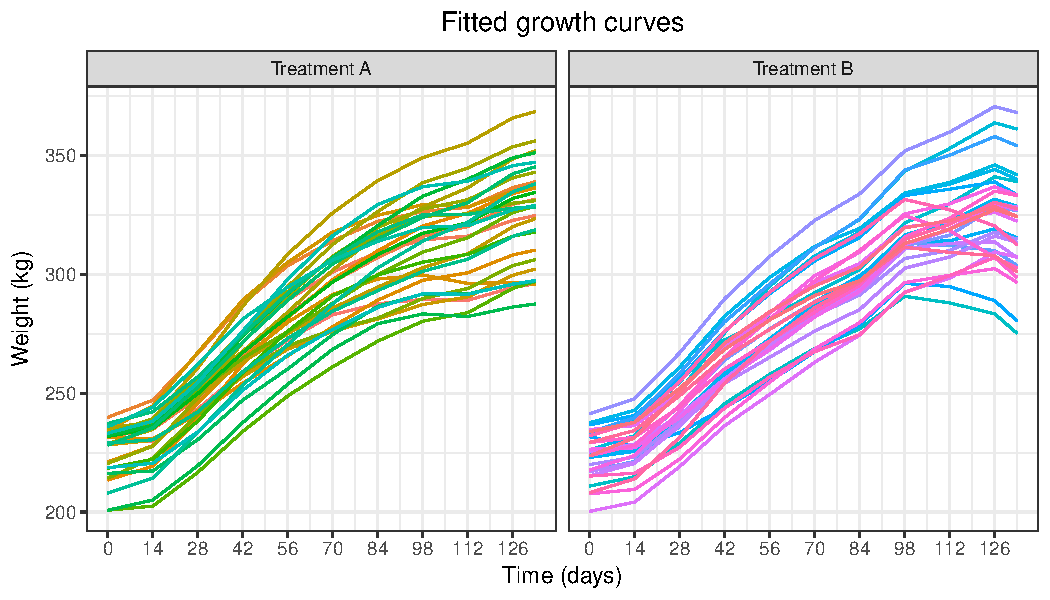
\includegraphics[width=\linewidth]{figure/cow_plot-1} 

}

\caption[A plot of the I-prior fitted regression curves from Model 5]{A plot of the I-prior fitted regression curves from Model 5. In this model, growth curves differ among cows and by treatment effect (with an interaction between cows and treatment effect), thus producing these 60 individual lines, one for each cow.}\label{fig:cow_plot}
\end{figure}


\end{knitrout}

We can next investigate whether the treatment effect differs among cows by comparing Model 5 against Model 4. As these models have the same number of parameters, we can simply choose the one with the higher likelihood, which is Model 5. We conclude that treatment does indeed have an effect on growth, and that the treatment effect differs among cows. We can use the \code{plot} function to plot the fitted regression curves onto the cow data set. This is shown in Figure \ref{fig:cow_plot}.

\end{document}


